\documentclass[10pt,polish]{beamer}

\usepackage[utf8x]{inputenc}
\usepackage[OT4]{fontenc}

\setbeamertemplate{navigation symbols}{}

\usetheme[bullet=circle,
          titleline=true,
          pageofpages=z,
          alternativetitlepage=true]{Torino}

\usepackage{ragged2e}
\usepackage{hyphenat}
\usepackage{hyperref}
\usepackage{booktabs}
\usepackage{listings}
\usepackage{multibib}

\usepackage{tikz}
\usepackage{pgfplots}

\usetikzlibrary{arrows}
\usetikzlibrary{automata}
\usetikzlibrary{backgrounds}
\usetikzlibrary{decorations}

\usepackage{amsmath}
\usepackage{amsfonts}
\usepackage{amsthm}

\usepackage{highlight/pythonhighlight}

\title{SymPy --- czyli matematyka w Pythonie}
\author{Mateusz Paprocki \texttt{<mattpap@gmail.com>}}
\institute{Wrocław University of Technology \\ University of Nevada, Reno}
\date{\today}

\newenvironment{jblock}[1]{
    \begin{block}{#1}\justifying\nohyphens
}{
    \end{block}
}

\setbeamercovered{transparent}

\begin{document}

\begin{frame}[plain,t]
    \maketitle
\end{frame}

\begin{frame}
    \frametitle{Plan prezentacji}
    \framesubtitle{}

    \begin{itemize}
        \item
    \end{itemize}
\end{frame}

\begin{frame}[fragile]
    \frametitle{Co to jest SymPy?}

    \begin{itemize}
        \item A \structure{pure Python library} for \structure{symbolic mathematics}
    \end{itemize}
    \pause
    \begin{python}
>>> from sympy import *
>>> x = Symbol('x')

>>> limit(sin(pi*x)/x, x, 0)
pi

>>> integrate(x + sinh(x), x)
(1/2)*x**2 + cosh(x)

>>> diff(_, x)
x + sinh(x)
    \end{python}
\end{frame}

\begin{frame}[fragile]
    \frametitle{How to get involved?}

    \begin{itemize}
        \item Visit our main web site:
            \begin{itemize}
                \item \texttt{www.sympy.org}
            \end{itemize}
        \item and additional web sites:
            \begin{itemize}
                \item \texttt{docs.sympy.org}
                \item \texttt{wiki.sympy.org}
                \item \texttt{live.sympy.org}
            \end{itemize}
        \item Contact us on our mailing list:
            \begin{itemize}
                \item \texttt{sympy@googlegroups.com}
            \end{itemize}
        \item or/and IRC channel:
            \begin{itemize}
                \item \texttt{\#sympy} on FreeNode
            \end{itemize}
        \item Clone source repository:
        \begin{verbatim}
        git clone git://github.com/sympy/sympy.git
        \end{verbatim}
    \end{itemize}
\end{frame}

\begin{frame}
    \frametitle{Moja rola w projekcie}
    \framesubtitle{Czyli odrobina historii z moim udziałem}

    \begin{itemize}
        \item początek współpracy w marcu 2007 roku
            \begin{itemize}
                \item kilka prostych poprawek i rozszerzeń
            \end{itemize}
            \pause
        \item następnie Google Summer of Code 2007
            \begin{itemize}
                \item algorytmy rozwiązywania równań rekurencyjnych
                \item algorytmy sumowania nieznaczonego i oznaczonego
            \end{itemize}
            \pause
        \item no i tak już zostało:
            \begin{itemize}
                \item algorytmy całkowania symbolicznego
                \item struktury algebraiczne, wielomiany
                \item upraszczanie wyrażeń, \ldots
            \end{itemize}
            \pause
        \item poza tym:
            \begin{itemize}
                \item Google Summer of Code 2009, 2010 mentor (PSU, PSF)
                \item EuroSciPy 2009 and 2010, py4science (UC Berkeley)
                \item praca dyplomowa
            \end{itemize}
    \end{itemize}
\end{frame}

\begin{frame}[fragile]
    \frametitle{Why polynomials not expressions?}
    \framesubtitle{}

    \begin{itemize}
        \item take advantage of
            \begin{itemize}
                \item additional knowledge
                    \begin{itemize}
                        \item monomial orderings, \ldots
                    \end{itemize}
                \item dedicated data structures
                \item polynomials manipulation algorithms
            \end{itemize}
        \pause
        \item efficiency concerns
            \begin{python}
In [1]: var('x')

In [2]: f = Add(*[ k*x**k for k in xrange(1, 1000) ])

In [3]: %timeit f + 3*f;
1 loops, best of 3: 773 ms per loop

In [4]: F = Poly(f, expand=False)

In [5]: %timeit F + 3*F;
100 loops, best of 3: 12.8 ms per loop
            \end{python}
    \end{itemize}
\end{frame}

\begin{frame}[fragile]
    \frametitle{Module's functionality}
    \framesubtitle{}

    \begin{itemize}
        \item classical arithmetics
        \item GCD, LCM, cofactors
        \item functional decomposition
        \item square--free decomposition
        \item factorization into irreducibles
        \item root counting, isolation, finding
        \item Gr\"{o}bner bases, monomial orderings
        \item polynomial remainder sequences
        \item subresultants, resultant, discriminant
        \item special polynomials
        \item polynomial forms
        \item \structure{\ldots}
    \end{itemize}
\end{frame}

\begin{frame}[fragile]
    \frametitle{Module's functionality}
    \framesubtitle{Factorization of polynomials}

    \begin{itemize}
        \item finite fields
            \begin{python}
In [1]: factor(x**2 + 1, modulus=2)
Out[1]: (1 + x)**2
            \end{python}
        \item rational numbers
            \begin{python}
In [2]: factor(x**6 + 1)
Out[2]: (1 + x**2)*(1 - x**2 + x**4)

In [3]: factor(expand((x + 101*y + 703*z)**20))
Out[3]: (x + 101*y + 703*z)**20
            \end{python}
        \item algebraic numbers
            \begin{python}
In [4]: factor(x**4 + 1, extension=I)
Out[4]: (I + x**2)*(-I + x**2)

In [5]: factor(x**2 - 2*y**2, extension=sqrt(2))
Out[5]: (x + y*2**(1/2))*(x - y*2**(1/2))
            \end{python}
    \end{itemize}
\end{frame}

\begin{frame}[fragile]
    \frametitle{Module's functionality}
    \framesubtitle{Solving inequalities}

    \begin{itemize}
        \item inequalities
            \begin{python}
In [1]: a = Symbol('a', real=True)

In [2]: solve(a**2 - 2 > 0, a)
Out[2]: [(-oo, -2**(1/2)), (2**(1/2), oo)]
            \end{python}
        \item systems of inequalities
            \begin{python}
In [3]: solve([a**2 - 2 < 0, a**2 - 1 > 0], a)
Out[3]: [(-2**(1/2), -1), (1, 2**(1/2))]
            \end{python}
        \item relational syntax
            \begin{python}
In [4]: solve([a**2 - 2 < 0, a**2 - 1 > 0], a, relational=True)
Out[4]: Or(And(-2**(1/2) < a, a < -1), And(1 < a, a < 2**(1/2)))
            \end{python}
        \item symbolic roots
            \begin{python}
In [5]: solve(a**5 + 2*a**3 + 3*a + 4 > 0, a)
Out[5]: [(RootOf(a**5 + 2*a**3 + 3*a + 4, 0), oo)]
            \end{python}
    \end{itemize}
\end{frame}

\begin{frame}[fragile]
    \frametitle{Module's functionality}
    \framesubtitle{Gr\"{o}bner bases and monomial orderings}

    \begin{itemize}
        \item monomial orderings
            \begin{python}
In [1]: LT(x*y**7 + 2*x**2*y**3, order='lex')
Out[1]: 2*x**2*y**3

In [2]: LT(x*y**7 + 2*x**2*y**3, order='grlex')
Out[2]: x*y**7
            \end{python}
        \item Gr\"{o}bner bases
            \begin{python}
In [3]: var('x1,x2,i1,i2,i3')
Out[3]: (x1, x2, i1, i2, i3)

In [4]: f1, f2, f3 = x1**2 + x2**2, x1**2*x2**2, x1**3*x2 - x1*x2**3

In [5]: G = groebner([f1 - i1, f2 - i2, f3 - i3], wrt='x1,x2')

In [6]: reduced(x1**7*x2 - x1*x2**7, G, wrt=[x1, x2])[1]
Out[6]: -i2*i3 + i3*i1**2

In [7]: _.subs({i1: f1, i2: f2, i3: f3}).expand()
Out[7]: x2*x1**7 - x1*x2**7
            \end{python}
    \end{itemize}
\end{frame}

\begin{frame}[fragile]
    \frametitle{Module's functionality}
    \framesubtitle{Generating special polynomials}

    \begin{itemize}
        \item symmetric polynomials
            \begin{python}
In [1]: symmetric_poly(2, x, y, z)
Out[1]: x*y + x*z + y*z
            \end{python}
        \item cyclotomic polynomials
            \begin{python}
In [2]: cyclotomic_poly(10, x)
Out[2]: 1 - x + x**2 - x**3 + x**4
            \end{python}
        \item orthogonal polynomials
            \begin{python}
In [3]: hermite_poly(6, x)
Out[3]: -120 + 720*x**2 - 480*x**4 + 64*x**6
            \end{python}
        \item Swinnerton--Dyer polynomials
            \begin{python}
In [4]: swinnerton_dyer_poly(3, x)
Out[4]: 576 - 960*x**2 + 352*x**4 - 40*x**6 + x**8
            \end{python}
    \end{itemize}
\end{frame}

\begin{frame}[fragile]
    \frametitle{Module's functionality}
    \framesubtitle{Polynomial forms: Horner}

    \begin{itemize}
        \item univariate polynomials
            \begin{python}
In [1]: horner(x**6 + 2*x**3 + 3*x**2 + 4*x + 5)
Out[1]: 5 + x*(4 + x*(3 + x*(2 + x**3)))

In [2]: horner(a*x**6 + b*x**3 + c*x**2 + d*x + e, x)
Out[2]: e + x*(d + x*(c + x*(b + a*x**3)))
            \end{python}
        \item multivariate polynomials
            \begin{python}
In [3]: sum(i*j*x**i*y**j, (i, 1, 2), (j, 1, 2))
Out[3]: x*y + 2*x*y**2 + 2*y*x**2 + 4*x**2*y**2

In [4]: horner(_3)
Out[4]: x*(y*(1 + 2*y) + x*y*(2 + 4*y))

In [5]: horner(_3, wrt=y)
Out[5]: y*(x*(1 + 2*x) + x*y*(2 + 4*x))
        \end{python}
    \end{itemize}
\end{frame}

\begin{frame}[fragile]
    \frametitle{Module's functionality}
    \framesubtitle{Computing symmetric reduction}

    \begin{itemize}
        \item symmetric polynomials
            \begin{python}
In [1]: symmetrize(x**2 + y**2)
Out[1]: (-2*x*y + (x + y)**2, 0)

In [2]: symmetrize(x**2 + y**2, formal=True)
Out[2]: (-2*s2 + s1**2, 0, {s1: x + y, s2: x*y})
            \end{python}
        \item non--symmetric polynomials
            \begin{python}
In [3]: symmetrize(x**2 - y**2)
Out[3]: (-2*x*y + (x + y)**2, -2*y**2)

In [4]: symmetrize(x**2 - y**2, formal=True)
Out[4]: (-2*s2 + s1**2, -2*y**2, {s1: x + y, s2: x*y})
            \end{python}
    \end{itemize}
\end{frame}

\begin{frame}
    \frametitle{Implemented algorithms}
    \framesubtitle{Only most remarkable cases here}

    \begin{itemize}
        \item square--free decomposition
            \begin{itemize}
                \item Yun
            \end{itemize}
        \item factorization into irreducibles
            \begin{itemize}
                \item finite fields
                    \begin{itemize}
                        \item Berlekamp, Zassenhaus, Shoup
                    \end{itemize}
                \item rational numbers
                    \begin{itemize}
                        \item Cantor--Zassenhaus, Wang
                    \end{itemize}
            \end{itemize}
        \item functional decomposition
            \begin{itemize}
                \item Landau--Zippel
            \end{itemize}
        \item Gr\"{o}bner bases
            \begin{itemize}
                \item Buchberger
            \end{itemize}
        \item root isolation
            \begin{itemize}
                \item continued fractions, Collins--Krandick
            \end{itemize}
    \end{itemize}
\end{frame}

\begin{frame}
    \frametitle{Use cases of the module}
    \framesubtitle{And SymPy in general}

    \begin{itemize}
        \item solving \structure{mathematical} problems
            \begin{itemize}
                \item e.g. in teaching mathematics
                \item Why?
                    \begin{itemize}
                        \item uses single, easy to learn programming language
                        \item core algorithms exposed to the user
                    \end{itemize}
                \item Example: graph $k$--coloring
            \end{itemize}
        \pause
        \item \structure{embedding} in other software
            \begin{itemize}
                \item e.g. code generation, preprocessing
                \item Why?
                    \begin{itemize}
                        \item small library with no dependencies
                    \end{itemize}
                \item Example: C code generation
            \end{itemize}
    \end{itemize}
\end{frame}

\begin{frame}
    \frametitle{Use cases of the module}
    \framesubtitle{Graph $k$--coloring with Gr\"{o}bner bases (1)}

    \begin{columns}
        \begin{column}[l]{0.4\textwidth}
            \begin{center}
                \includegraphics<1->[scale=0.6]{images/graph-nocolor.pdf}
            \end{center}
        \end{column}
        \begin{column}[r]{0.4\textwidth}
            \begin{center}
                \includegraphics<2->[scale=0.6]{images/graph-color.pdf}
            \end{center}
        \end{column}
    \end{columns}
\end{frame}

\begin{frame}
    \frametitle{Use cases of the module}
    \framesubtitle{Graph $k$--coloring with Gr\"{o}bner bases (2)}

    Given a graph $\mathcal{G}(V, E)$ we write two sets of equations:
    \begin{itemize}
        \pause
        \item $I_k$ --- allow one of $k$ colors per vertex
            \begin{equation*}
                I_k = \{ x_i^k - 1 : i \in V \}
            \end{equation*}
        \pause
        \item $I_{\mathcal{G}}$ --- adjacent vertices have different colors assigned
            \begin{equation*}
                I_{\mathcal{G}} = \{ x_{i}^{k-1} + x_{i}^{k-2} x_{j} + \ldots + x_{i} x_{j}^{k-2} + x_{j}^{k-1} : (i, j) \in E \}
            \end{equation*}
    \end{itemize}
    \pause
    Next we solve $I_k \cup I_{\mathcal{G}}$ using the Gr\"{o}bner bases method.
\end{frame}

\begin{frame}
    \frametitle{Use cases of the module}
    \framesubtitle{Graph $k$--coloring with Gr\"{o}bner bases (3)}

    \begin{columns}
        \begin{column}[l]{0.4\textwidth}
            \begin{align*}
                \{& \structure{x_{1}} + x_{11} + x_{12},              \\
                  & \structure{x_{2}} - x_{11},                       \\
                  & \structure{x_{3}} - x_{12},                       \\
                  & \structure{x_{4}} - x_{12},                       \\
                  & \structure{x_{5}} + x_{11} + x_{12},              \\
                  & \structure{x_{6}} - x_{11},                       \\
                  & \structure{x_{7}} - x_{12},                       \\
                  & \structure{x_{8}} + x_{11} + x_{12},              \\
                  & \structure{x_{9}} - x_{11},                       \\
                  & \structure{x_{10}} + x_{11} + x_{12},             \\
                  & \structure{x_{11}}^2 + x_{11} x_{12} + x_{12}^2,  \\
                  & \structure{x_{12}}^3 - 1 \}
            \end{align*}
        \end{column}
        \begin{column}[r]{0.4\textwidth}
            \begin{center}
                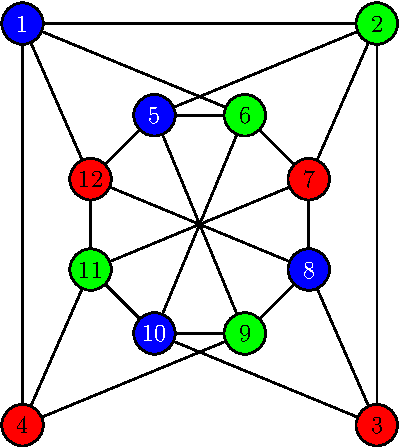
\includegraphics[scale=0.6]{images/graph-color.pdf}
            \end{center}
        \end{column}
    \end{columns}
\end{frame}

\begin{frame}[fragile]
    \frametitle{Use cases of the module}
    \framesubtitle{Graph $k$--coloring with Gr\"{o}bner bases (4)}

    Here is how to solve \structure{$3$--coloring} problem in SymPy:
    \begin{python}
In [1]: V = range(1, 12+1)
In [2]: E = [(1,2),(2,3),(1,4),(1,6),(1,12),(2,5),(2,7),
(3,8),(3,10),(4,11),(4,9),(5,6),(6,7),(7,8),(8,9),(9,10),
(10,11),(11,12),(5,12),(5,9),(6,10),(7,11),(8,12)]

In [3]: X = [ Symbol('x' + str(i)) for i in V ]
In [4]: E = [ (X[i-1], X[j-1]) for i, j in E ]

In [5]: I3 = [ x**3 - 1 for x in X ]
In [6]: Ig = [ x**2 + x*y + y**2 for x, y in E ]

In [7]: G = groebner(I3 + Ig, X, order='lex')

In [8]: G != [1]
Out[8]: True
    \end{python}
\end{frame}

\begin{frame}[fragile]
    \frametitle{Use cases of the module}
    \framesubtitle{Graph $k$--coloring with Gr\"{o}bner bases (4)}

    \begin{figure}
        \begin{center}
            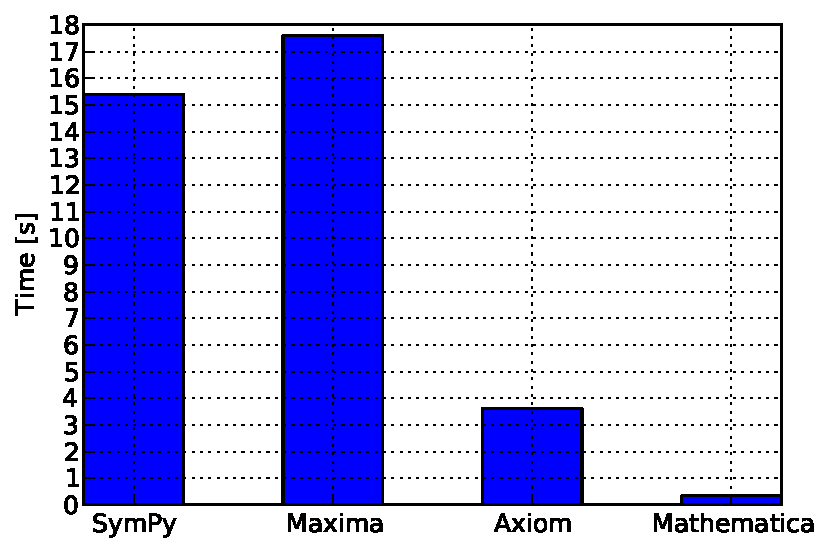
\includegraphics[scale=0.55]{images/groebner-time-compare.pdf}
        \end{center}
        \caption{Average timing of Gr\"{o}bner basis computation}
    \end{figure}
\end{frame}

\begin{frame}[fragile]
    \frametitle{Use cases of the module}
    \framesubtitle{C code generation (1)}

    The problem:
    \begin{itemize}
        \item transform expressions into \structure{Horner form}
        \item generate equivalent \structure{C code}
            \begin{itemize}
                \item e.g. for fast evaluation
            \end{itemize}
        \item assume we can't use \texttt{pow()} function
    \end{itemize}
    \vskip+0.5cm
    \pause
    How we will approach the problem?
    \begin{itemize}
        \item define a new \structure{printer} to generate code
        \item use \texttt{horner()} to transform expressions
    \end{itemize}
\end{frame}

\begin{frame}[fragile]
    \frametitle{Use cases of the module}
    \framesubtitle{C code generation (2)}

    Lets define a dedicated \structure{printer} for the task:
    \begin{python}
from sympy.printing import StrPrinter

class CPrinter(StrPrinter):
    """Print Lambda as C function and unroll Pow. """

    counter = 0

    def _print_Lambda(self, expr):
        self.counter += 1

        return """long _L%i(long %s) {\n  return (%s);\n}""" % \
            (self.counter, expr.args[0], self.doprint(expr.args[1]))

    def _print_Pow(self, expr):
        if expr.exp.is_Integer:
            return '*'.join([str(expr.base)]*int(expr.exp))
        else:
            return StrPrinter._print_Pow(self, expr)
    \end{python}
\end{frame}

\begin{frame}[fragile]
    \frametitle{Use cases of the module}
    \framesubtitle{C code generation (3)}

    Lets \structure{generate} some \structure{code} using the new \texttt{CPrinter}:
    \begin{python}
In [1]: from sympy import horner, Lambda

In [2]: from sympy.abc import x

In [3]: f = horner(x**6 + 2*x**3 + 3*x**2 + 4*x + 5)

In [4]: print CPrinter().doprint(Lambda(x, f))
Out[4]:
double _L1(double _x) {
  return (5 + (4 + (3 + (2 + _x*_x*_x)*_x)*_x)*_x);
}
    \end{python}
\end{frame}

\begin{frame}[fragile]
    \frametitle{Pure mode Cython}
    \framesubtitle{}

    Why want to use \structure{Cython}?
    \begin{itemize}
        \item we want speed improvements
        \item we don't want to write C/C++ by hand
    \end{itemize}
    \pause
    Why we want to use \structure{pure mode} Cython?
    \begin{itemize}
        \item actually we don't want to write Cython either
        \item allows us to have a single source base
        \item it is very cheap to use
    \end{itemize}
\end{frame}

\begin{frame}[fragile]
    \frametitle{Using pure mode Cython}
    \framesubtitle{How to use pure mode Cython in SymPy?}

    \begin{itemize}
        \item install Cython (\texttt{www.cython.org}) on your system
        \pause
        \item annotate selected functions with \texttt{cythonized} decorator
        \pause
        \item choose which variables should be considered as native
        \pause
        \item type \texttt{make} in your shell and rerun SymPy
    \end{itemize}
    \pause
    Example:
    \begin{python}
@cythonized('i,n')
def dup_scale(f, a, K):
    """Compute ``f(a*x)`` in ``K[x]``. """
    f, n, b = list(f), dup_degree(f), a

    for i in xrange(n-1, -1, -1):
        f[i], b = b*f[i], b*a

    return f
    \end{python}
\end{frame}

\begin{frame}[fragile]
    \frametitle{Using pure mode Cython}
    \framesubtitle{How \texttt{cythonized} decorator works?}

    \begin{itemize}
        \item \structure{with} Cython
            \begin{python}
def cythonized(specs):
    arg_types = {}

    for spec in specs.split(','):
        arg_types[spec] = cython.int

    return cython.locals(**arg_types)
            \end{python}
        \pause
        \item \structure{without} Cython
            \begin{python}
def cythonized(specs):
    return lambda f: f
            \end{python}
    \end{itemize}
\end{frame}

\begin{frame}
    \frametitle{Plany na przyszłość}
    \framesubtitle{}

    \begin{itemize}
        \item
    \end{itemize}
\end{frame}

\begin{frame}
    \frametitle{Dziękuję za uwagę!}
    \framesubtitle{Pytania, uwagi, dyskusja \ldots}

    \begin{center}
        
\includegraphics[scale=0.2]{images/sympy-logo.pdf}
    \end{center}
\end{frame}

\end{document}

